\documentclass[a4paper,12pt]{article}

% Pakete für PDF-Hintergrund
\usepackage{eso-pic}
\usepackage{graphicx}
\usepackage{geometry}

% Seitenränder anpassen
\geometry{
    top=2cm,
    bottom=2cm,
    left=2cm,
    right=2cm
}

% Deutsche Sprachunterstützung
\usepackage[ngerman]{babel}
\usepackage[utf8]{inputenc}
\usepackage[T1]{fontenc}

% Schriftart für LuaLaTeX
\usepackage{fontspec}
\setmainfont{Chalkboard}[
    Extension = .ttc,
    UprightFont = *,
    BoldFont = *,
    ItalicFont = *,
    BoldItalicFont = *
]

% Mathematik-Pakete
\usepackage{amsmath}
\usepackage{amssymb}

% Anführungszeichen für Bibliographie
\usepackage{csquotes}

% Bibliographie mit Biber
\usepackage[backend=biber,style=numeric,sorting=none]{biblatex}
\addbibresource{bibliography.bib}

% PDF als Hintergrund einbinden
\AddToShipoutPictureBG{%
    \AtPageLowerLeft{%
        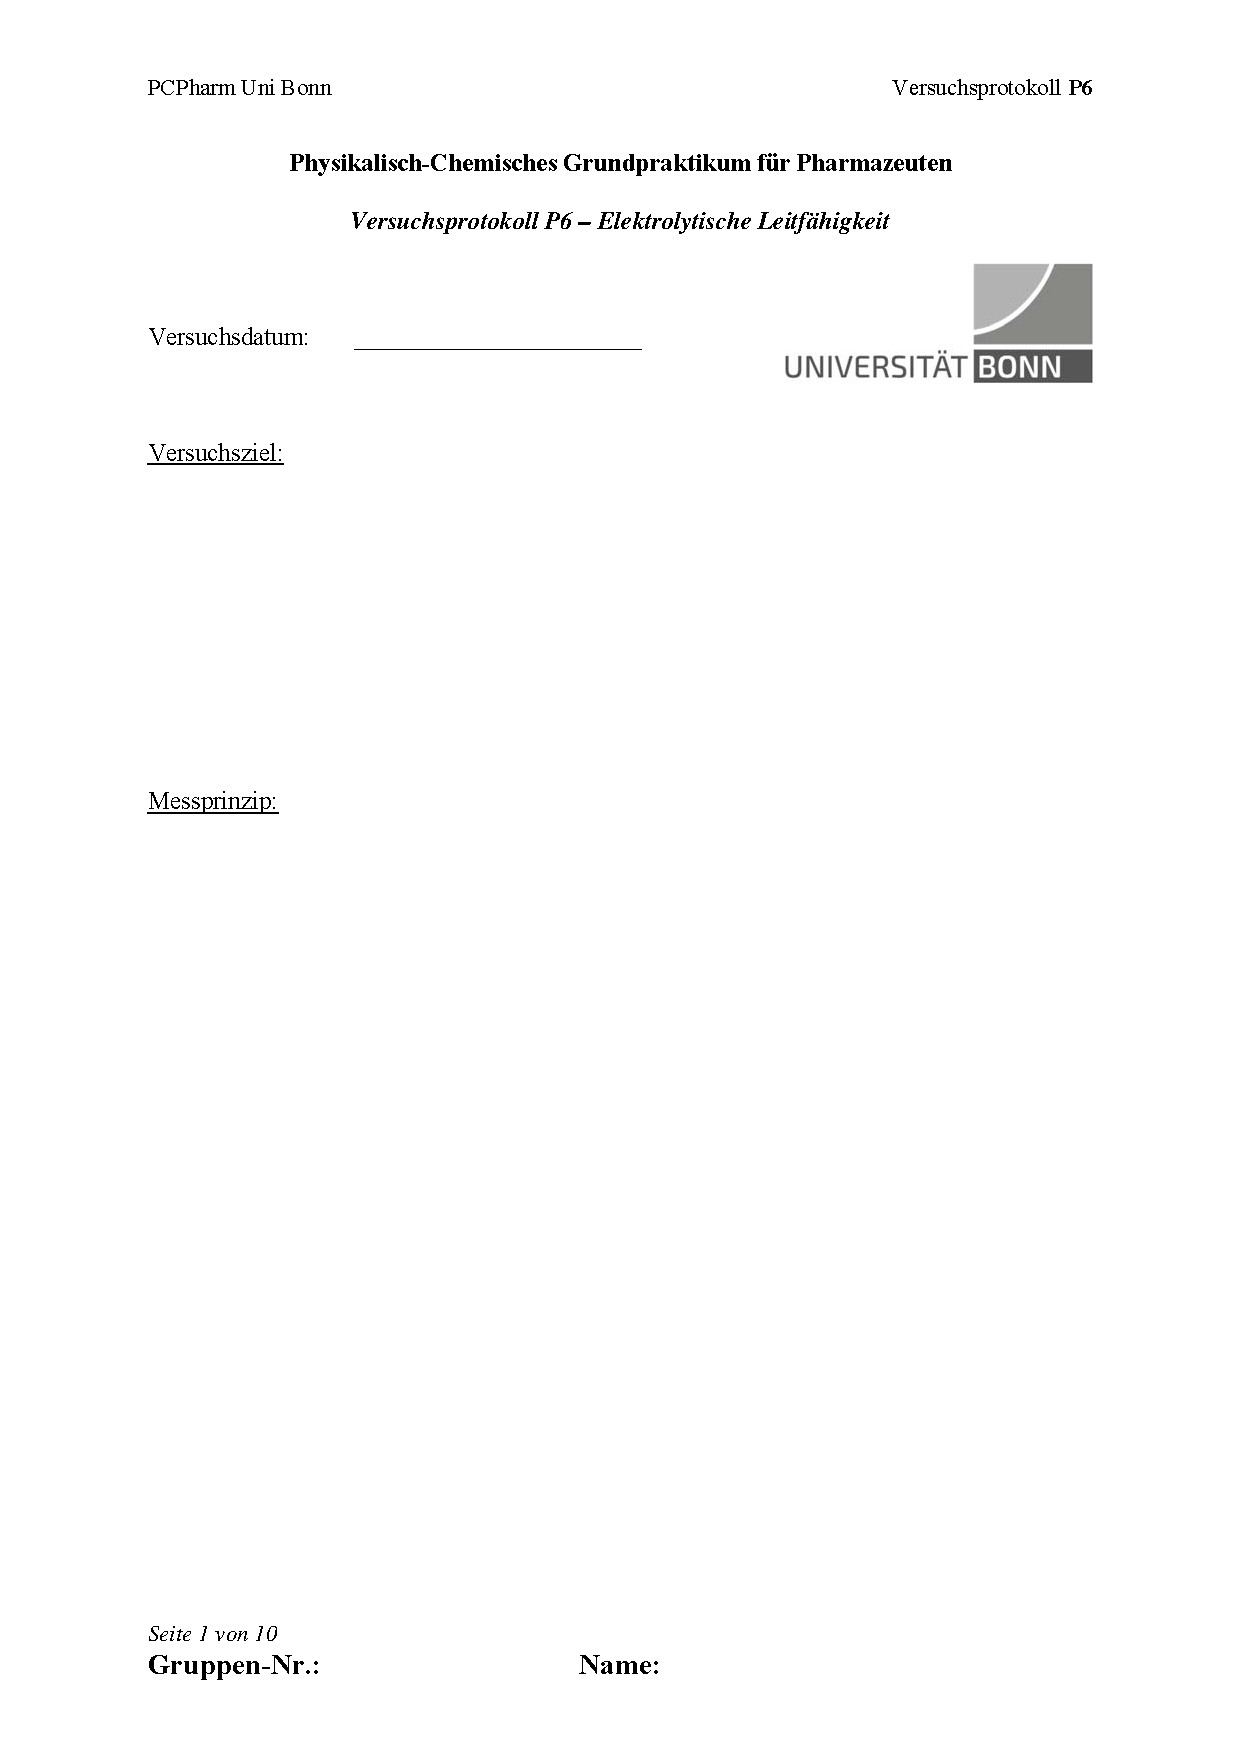
\includegraphics[width=\paperwidth,height=\paperheight]{Protokoll P6 PC Ph SS2022.pdf}%
    }%
}

% Transparenter Text für bessere Lesbarkeit
\usepackage{xcolor}
\usepackage{transparent}

\parindent=0pt % Keine Einrückung bei neuen Absätzen

\begin{document}

% Optional: Textfarbe anpassen für bessere Sichtbarkeit

\color{white}
.\newline

\vspace{5.5cm}

\color{blue}
Die Identität eines schwachen Elektrolyten und eines starken Elektrolyten sollen konduktometrisch bestimmt werden. Dafür sollen die Grenzleitfähigkeit $\Lambda^\infty$, die Dissoziationskonstante $K_c^{\text{app}}$ sowie der negative dekadische Logarithmus der Dissoziationskonstanten $\text{p}K_c^{\text{app}}$ des schwachen Elektrolyten und die Konstante $k$ sowie die Grenzleitfähigkeit $\Lambda^\infty$ des starken Elektrolyten bestimmt werden.

\vspace{3.5cm}

Die Leitfähigkeitsmessung der temperierten Elektrolytlösungen, welche als Verdünnungsreihe hergestellt werden, erfolgt mittels einer Kohlrauschschen-Leitfähigkeitsmesszelle und einer Wheatstoneschen Brückenschaltung. Die Wheatstonesche Brückenschaltung wird mit Wechselspannung betrieben, um Polarisation an den Elektroden zu vermeiden. Auf Grund der Wechselspannung wird die Brücke vollständig mittels eines Oszilloskops abgeglichen, wobei Ohmsche Widerstände und kapazitive Blindwiderstände berücksichtigt werden. In diesem Zustand kann der Widerstand $R$ bzw. der Leitwert $G$ der Elektrolytlösung aus den bekannten Widerständen der Wheatstoneschen Brücke berechnet werden.\\
Zur Bestimmung der Zellkonstanten $K_\mathrm{Z}$ wird eine Zweipunktkalibrierung mit einer KCl-Kalibrierlösung bekannter Leitfähigkeit $\kappa$ durchgeführt.\\ \\
Aus diesen Werten können die Leitfähigkeiten $\kappa$, welche um die Leitfähigkeit des verwendeten Wassers korrigiert werden, und die Äquivalenzleitfähigkeiten $\Lambda$ berechnet werden.\\ \\
Für den schwachen Elektrolyten können nach dem Ostwaldschen Verdünnungsgesetz die linearisierten Auftragungen $\Lambda=f(\Lambda^2c)$ und $\Lambda^{-1}=f(\Lambda c)$ erstellt werden, wodurch $\Lambda^\infty$, $K_c^{\text{app}}$ und $\text{p}K_c^{\text{app}}$ bestimmt werden können. Für den starken Elektrolyten wird nach dem Kohlrauschschen Quadratwurzelgesetz die linearisierte Auftragung $\Lambda=f(c^{1/2})$ erstellt, wodurch die Konstante $k$ und die Grenzleitfähigkeit $\Lambda^\infty$ bestimmt werden können.\\ \\
Durch den Vergleich der experimentell bestimmten Werte mit Literaturwerten können die Elektrolytlösungen identifiziert werden.
    
\end{document}